\begin{example}[Mnożenie macierzy]
	\begin{flalign*}
		A,\ B \text{ - macierze } n\times n &  &  & A\cdot B = C = ? &  &  &
	\end{flalign*}
	\begin{minipage}{0.6\linewidth}
		Najpopularniejszy sposób mnożenia dwóch macierzy $n\times n$ działa w czasie $\BO(n^3)$.
		Musimy obliczyć $n^2$ wartości i obliczenie każdej zajmuje liniowy czas.
	\end{minipage}\hfill\begin{minipage}{0.35\linewidth}
		\begin{flalign*}
			\begin{array}{rl}
				B = & \left[\begin{array}{c} \vdots \end{array}\right]     \\[2ex]
				A = \left[\begin{array}{cc} \cdots \end{array}\right]
				    & \left[\begin{array}{c} \times \end{array}\right] = C
			\end{array}
		\end{flalign*}
	\end{minipage}

	\subsection{Algorytm Strasiera}
	Zakładamy, że $n$ jest potęgą $2$ (dla przejrzystości). Dzielimy $A$ i $B$ na $4$ macierze $\frac{n}{2}\times \frac{n}{2}$:

	\begin{flalign*}
		                                           & A = \begin{bNiceArray}{cc}[margin,hvlines]
			                                                 A_{11} & A_{12} \\
			                                                 A_{21} & A_{22}
		                                                 \end{bNiceArray},\
		B = \begin{bNiceArray}{cc}[margin,hvlines]
			    B_{11} & B_{12} \\
			    B_{21} & B_{22}
		    \end{bNiceArray} &                                                               &  &  &                                            \\
		%
		                                           & A\cdot B = \begin{bNiceArray}{cc}[margin,hvlines]
			                                                        A_{11} & A_{12} \\
			                                                        A_{21} & A_{22}
		                                                        \end{bNiceArray} \cdot \begin{bNiceArray}{cc}[margin,hvlines]
			                                                                               B_{11} & B_{12} \\
			                                                                               B_{21} & B_{22}
		                                                                               \end{bNiceArray} = \begin{bNiceArray}{cc}[margin,hvlines]
			                                                                                                  C_{11} & C_{12} \\
			                                                                                                  C_{21} & C_{22}
		                                                                                                  \end{bNiceArray} &  &  &   & \\
		%
		                                           & C_{11} = A_{11}B_{11} + A_{12}B_{21}                          &  &  &   &                  \\
		                                           & C_{12} = A_{11}B_{12} + A_{12}B_{22}                          &  &  &   &                  \\
		                                           & C_{21} = A_{21}B_{11} + A_{22}B_{21}                          &  &  &   &                  \\
		                                           & C_{22} = A_{21}B_{12} + A_{22}B_{22}                          &  &  &   &
	\end{flalign*}

	Zamieniliśmy $1$ mnożenie macierzy $n\times n$ na $8$ mnożeń macierzy $\frac{n}{2}\times \frac{n}{2}$ + podział i dodawanie ($\BO(n^2)$).
	Stąd mamy zależność rekurencyjną:
	\begin{flalign*}
		T(n) & = 8\cdot T(\frac{n}{2}) + \BT(n^2)                                          &  & a = 8,\ b = 2,\ k = 2 &  & \\[1.5ex]
		8    & > 2^2 \Rightarrow T(n) = \BT\left(n^{\log_2 8}\right) = \BT\left(n^3\right) &  &                       &  &
	\end{flalign*}

	Strassen zauważył, że jeśli obliczymy
	\begin{flalign*}
		 & M_{1} = (A_{12} - A_{22})\cdot (B_{21} + B_{22}) &  &  &            &                                \\
		 & M_{2} = (A_{11} + A_{22})\cdot (B_{11} + B_{22}) &  &  & \text{to } & C_{11} = M_1 + M_2 - M_4 + M_6 \\
		 & M_{3} = (A_{11} - A_{21})\cdot (B_{11} + B_{12}) &  &  &            & C_{12} = M_4 + M_5             \\
		 & M_{4} = (A_{11} + A_{12})\cdot B_{22}            &  &  &            & C_{21} = M_6 + M_7             \\
		 & M_{5} = A_{11}\cdot (B_{12} - B_{22})            &  &  &            & C_{22} = M_2 - M_3 + M_5 - M_7 \\
		 & M_{6} = A_{22}\cdot (B_{21} - B_{11})            &  &  &            &                                \\
		 & M_{7} = (A_{21} + A_{22})\cdot B_{11}            &  &  &            &
	\end{flalign*}

	Zatem
	\begin{flalign*}
		T(n) & = 7\cdot T\left(\frac{n}{2}\right) + \BT(n^2)                                    &  & a = 7,\ b = 2,\ k = 2 &  & \\[1.5ex]
		7    & > 2^2 \Rightarrow T(n) = \BT\left(n^{\log_2 7}\right) = \BT\left(n^{2.81}\right) &  &                       &  &
	\end{flalign*}
\end{example}

\subsection{Własność optymalnej podstruktury}
Optymalne rozwiązanie problemu jest funkcją optymalnych rozwiązań podproblemów
(optymalne rozwiązanie można skonstruować z optymalnych rozwiązań podproblemów).
Żeby metoda \textit{dziel i zwyciężaj} działała dobrze muszą być spełnione dwa warunki (przez problem i algorytm):
\begin{enumerate}
	\item własność optymalnej podstruktury
	\item podproblemy są rozłączne
\end{enumerate}

\subsection{Znajdywanie pary najbliższych punktów}
$Q$ - zbiór $n \geq 2$ punktów na płaszczyźnie
\begin{flalign*}
	p_1 = (x_1, y_1) &  & p_2 = (x_2, y_2) &  & d(p_1, p_2) = \sqrt{(x_1 - x_2)^2 + (y_1 - y_2)^2} &  &  &  &  &  &  &  &
\end{flalign*}
Problem: znaleźć parę punktów w najmniejszej odległości. Algorytm siłowy (\textit{brute force}), który
sprawdza wszystkie pary punktów działa w czasie $\BT(n^2)$, bo mamy $\binom{n}{2} = \frac{n(n - 1)}{2} = \BT(n^2) $ par punktów.
Pokażemy algorytm typu \textit{dziel i zwyciężaj}, który działa w czasie $\BO(n\log n)$.

W każdym wywołaniu rekurencyjnym wejście składa się z 3 rzeczy:
zbioru $P\subset Q$ i dwóch tablic $X$ i $Y$ które zawierają wszystkie punkty z $P$.
W tablicy $X$ punkty są posortowane w porządku niemalejącym względem pierwszej współrzędnej,
a w tablicy $Y$ po drugiej współrzędnej.

Opis algorytmu:
\begin{itemize}
	\item[jeśli $|P| \leq 3$] sprawdzamy wszystkie pary
	\item[jeśli $|P| > 3$] ~
	      \begin{itemize}
		      \item[\uemph{Dziel:}] Dzielimy punkty $P$ pionową prostą $l$ na dwa podzbiory $P_L$ i $P_R$ na lewo i na prawo
		            od $l$ tak, że $|P_L| = \left\lceil \frac{|P|}{2} \right\rceil,\ |P_R| = \left\lfloor \frac{|P|}{2} \right\rfloor$.
		            Dzielimy tablicę $X$ na $X_L$ i $X_R$ zawierające punkty odpowiednio $P_L$ i $P_R$ posortowane w porządku
		            niemalejącym względem pierwszej współrzędnej. Podobnie dzielimy $Y$ na $Y_L$ i $Y_R$ zawierające
		            odpowiednio punkty z $P_L$ i $P_R$ posortowane w porządku niemalejącym po drugiej współrzędnej.

		            \begin{figure}[ht]
			            \centering
			            \begin{tikzpicture}[>=stealth, font=\small, scale=0.8]
				            % pionowa prosta l dzielaca P
				            \draw[thick] (4,-0.4) -- (4,5.2);
				            \node[above] at (4,5.2) {$l$};

				            % etykiety P_L, P_R
				            \node at (1.7,5.0) {$P_L$};
				            \node at (6.3,5.0) {$P_R$};

				            % punkty na lewo od l (P_L)
				            \foreach \p in {(0.6,1.2),(1.4,3.6),(0.9,2.5),(2.2,0.8),%
						            (1.8,4.4),(3.1,2.0),(2.6,3.2),(3.4,1.0)}
				            \fill[accent] \p circle (2.6pt);

				            % punkty na prawo od l (P_R)
				            \foreach \p in {(4.7,3.8),(5.3,1.5),(6.1,2.9),(5.0,0.9),%
						            (6.8,3.5),(7.2,1.8),(5.8,4.3),(6.4,0.7)}
				            \fill[red!70!black] \p circle (2.6pt);
			            \end{tikzpicture}
			            \caption{Podział zbioru $P$ pionową prostą $l$ na podzbiory $P_L$
				            (na~lewo) i~$P_R$ (na~prawo) o~rozmiarach $|P_L| = \left\lceil \frac{|P|}{2} \right\rceil$
				            oraz $|P_R| = \left\lfloor \frac{|P|}{2} \right\rfloor$.}
			            \label{fig:closestpoints:split}
		            \end{figure}

		      \item[\uemph{Zwyciężaj:}] Wywołujemy rekurencyjnie algorytm dla wejścia $P_L,\ X_L,\ Y_L$ i $P_R,\ X_R,\ Y_R$.
		            Algorytm znajduje pary najbliższych punktów w $P_L$ i $P_R$. Niech $\delta_L$ i $\delta_R$ będą
		            najmniejszymi odległościami znalezionymi przez algorytm dla odpowiednio $P_L$ i $P_R$.
		            Niech $\delta$ będzie mniejszą z nich: $\delta = \min(\delta_L,\delta_R)$.

		      \item[\uemph{Połącz:}] Para najbliższych punktów z $P$ składa się z dwóch punktów z $P_L$ lub z dwóch punktów
		            z $P_R$ lub jednego punkty z $P_L$ i jednego z $P_R$.

		            Musimy sprawdzić czy istnieje para 3-go typu w odległości mniejszej niż $\delta$.
		            Jeśli taka para istnieje, wtedy jej punkty są w pionowym pasie o szerokości $2\delta$
		            wokół $l$.

		            W celu sprawdzenia czy taka para istnieje wykonujemy następujące czynności:
		            \begin{enumerate}
			            \item Tworzymy tablicę $Y'$ otrzymaną z $Y$ poprzez usunięcie punktów spoza pasa. $Y'$ jest
			                  posortowany w porządku niemalejącym względem drugiej współrzędnej.
			            \item Dla każdego punktu $p$ z $Y'$ sprawdzamy odległość między $p$, a $p'$ dla $7$ kolejnych
			                  punktów $p'$ z $Y'$. Algorytm oblicza najmniejszą odległość $\delta'$ i zapamiętuje ją i odpowiednią
			                  parę punktów.
			            \item Jeśli $\delta' < \delta$ to pionowy pas zawiera parę punktów w mniejszej odległości niż pary znalezione
			                  w wywołaniach rekurencyjnych. Algorytm zwraca $\delta'$ i odpowiednią parę punktów. Wpp. zwraca $\delta$
			                  i odpowiednią parę punktów.
		            \end{enumerate}
	      \end{itemize}
\end{itemize}

\begin{proof}[Dowód poprawności]
	Jedyną rzeczą, która nie jest oczywista jest fakt, że sprawdzamy tylko $7$ następnych punktów po $p$ w $Y'$ w fazie połącz.
	Przypuśćmy, że $p, q$ są parą punktów w najmniejszej odległości w $P$ i $d(p,q) = \delta'$. Niech
	$p = (x_p, y_p),\ q = (x_q, y_q)$. Bez straty ogólności załóżmy $y_p \leq y_q$. Pokażemy, że algorytm znajdzie
	tę parę punktów. Przypuśćmy, że nie. Wtedy istnieje co najmniej $7$ punktów pomiędzy $p$ i $q$ w $Y'$.
	Niech $r = (x_r, y_r)$ będzie jednym z nich. Skoro $d(p,q) < \delta$ to
	$y_q - y_p = |y_q - y_p| \leq \sqrt{(x_p - x_q)^2 + (y_p - y_q)^2} = d(p, q) < \delta$.
	Ponadto $y_r$ musi być między $y_p$ i $y_q$: $y_p \leq y_r \leq y_q$, więc $y_r - y_p \leq y_q - y_p < \delta$
	zatem co najmniej 9 punktów z $P$ w prostokącie $2\delta\times\delta$ ograniczonym poziomymi liniami
	$y = y_p,\ y = y_p + \delta$.

	\begin{figure}[ht]
		\centering
		\begin{tikzpicture}[>=stealth, font=\small, scale=0.9]
			\def\d{2} % delta

			% lewy kwadrat delta x delta (co najmniej 5 punktow)
			\fill[pattern=north east lines, pattern color=gray!70]
			(0,0) rectangle (\d,\d);

			% poziome proste y = y_p oraz y = y_p + delta
			\draw (-1.3,0)  -- (2*\d+0.6,0);
			\draw (-1.3,\d) -- (2*\d+0.6,\d);

			% pionowe proste x = x_L-d, x_L, x_L+d
			\draw (0,-1.5)    -- (0,2.4);
			\draw (\d,-2.1)   -- (\d,2.4);
			\draw (2*\d,-1.5) -- (2*\d,2.4);

			% etykiety P_L, P_R oraz szerokosci delta na gorze
			\node[above] at (\d/2,2.7)   {$P_L$};
			\node[above] at (3*\d/2,2.7) {$P_R$};
			\draw[decorate, decoration={brace, amplitude=4pt}]
			(0,2.05) -- (\d,2.05) node[midway, above=3pt] {$\delta$};
			\draw[decorate, decoration={brace, amplitude=4pt}]
			(\d,2.05) -- (2*\d,2.05) node[midway, above=3pt] {$\delta$};

			% wysokosc delta oraz etykiety y po prawej
			\draw[decorate, decoration={brace, amplitude=4pt}]
			(2*\d,\d) -- (2*\d,0) node[midway, right=4pt] {$\delta$};
			\node[right] at (2*\d+0.7,\d) {$y = y_p + \delta$};
			\node[right] at (2*\d+0.7,0) {$y = y_p$};

			% etykiety x na dole
			\node[below] at (0,-1.5)    {$x = x_L - \delta$};
			\node[below] at (\d,-2.1)   {$x = x_L$};
			\node[below] at (2*\d,-1.5) {$x = x_L + \delta$};
		\end{tikzpicture}
		\caption{Prostokąt $2\delta\times\delta$ ograniczony prostymi $y = y_p$ oraz
			$y = y_p + \delta$. Zacieniowany lewy kwadrat $\delta\times\delta$
			zawiera co najmniej $5$ punktów z~$P$.}
		\label{fig:closestpoints:rectangle}
	\end{figure}

	Wtedy w lewym lub prawym kwadracie $\delta\times\delta$ jest przynajmniej $5$ punktów z $P$. Przypuśćmy,
	że to lewy kwadrat. Zatem istnieje kwadrat $\delta\times\delta$ z $5$ punktami z $P$ w $P_L$.
	Ale wtedy istnieją dwa punkty w $P_L$ w odległości mniejszej niż $\delta$, bo nie da się umieścić
	w kwadracie $\delta\times\delta$ $5$ punktów dla których odległość między dowolnymi dwoma
	jest mniejsza niż $\delta$. Sprzeczność (bo najmniejsza odległość w $P_L$ to $\delta_L \geq \delta$).

	\begin{figure}[ht]
		\centering
		\begin{tikzpicture}[>=stealth, font=\small, scale=1.6]
			\def\d{2} % delta

			% kwadrat delta x delta
			\draw (0,0) rectangle (\d,\d);

			% podzial na cztery komorki delta/2 x delta/2
			\draw[gray, dotted] (\d/2,0) -- (\d/2,\d);
			\draw[gray, dotted] (0,\d/2) -- (\d,\d/2);

			% odcinki od srodkowego punktu do naroznikow (odleglosc delta/sqrt2 < delta)
			\foreach \c in {(0,0),(\d,0),(\d,\d),(0,\d)}
			\draw[red!70, dashed] (\d/2,\d/2) -- \c;

			% cztery punkty w naroznikach
			\foreach \c in {(0,0),(\d,0),(\d,\d),(0,\d)}
			\fill \c circle (1.6pt);

			% piaty punkt w srodku
			\fill[red] (\d/2,\d/2) circle (1.8pt);
			\node[red, below right=-1pt] at (\d/2,\d/2) {$q$};
			\node[red, above right=1pt] at (\d/4,3*\d/4) {$\tfrac{\delta}{\sqrt{2}}$};

			% szerokosc i wysokosc delta
			\draw[decorate, decoration={brace, amplitude=4pt}]
			(0,\d+0.1) -- (\d,\d+0.1) node[midway, above=3pt] {$\delta$};
			\draw[decorate, decoration={brace, amplitude=4pt}]
			(\d+0.1,\d) -- (\d+0.1,0) node[midway, right=4pt] {$\delta$};
		\end{tikzpicture}
		\caption{W kwadracie $\delta\times\delta$ nie zmieści się $5$ punktów parami
			oddalonych o co najmniej $\delta$. Najlepsze ułożenie to $4$ naroż\-niki;
			dowolny piąty punkt~$q$ jest w odległości co najwyżej $\frac{\delta}{\sqrt{2}}<\delta$
			od któregoś z nich (dwa z~$5$ punktów trafiają do tej samej ćwiartki
			$\frac{\delta}{2}\times\frac{\delta}{2}$).}
		\label{fig:closestpoints:fivepoints}
	\end{figure}

	Zatem wystarczy sprawdzić tylko $7$ następnych punktów po $p$ w $Y'$.
\end{proof}

\begin{dygresja}
	Powyższy dowód prowadzimy \emph{nie wprost}, ale tę samą granicę $7$ można dostać równie dobrze \emph{wprost}, zliczając punkty. Oba rozumowania korzystają z tego samego faktu geometrycznego (w~kwadracie $\delta\times\delta$ mieści się co najwyżej $4$ punkty parami oddalone o~co najmniej $\delta$) i~są równoważne -- różnią się jedynie sposobem zliczania.

	\textbf{Wersja wprost.} Ustalmy punkt $p$ z~$Y'$. Każdy punkt $p'$, którego odległość od $p$ chcemy sprawdzić, leży w~prostokącie $2\delta\times\delta$ ograniczonym pasem szerokości $2\delta$ wokół $l$ oraz liniami $y = y_p$ i~$y = y_p + \delta$ (bo $Y'$ jest posortowane względem~$y$, więc patrzymy tylko w~stronę rosnącego~$y$). Podzielmy ten prostokąt prostą~$l$ na lewy i~prawy kwadrat $\delta\times\delta$. Lewy kwadrat leży w~całości w~$P_L$, więc wszystkie jego punkty są parami oddalone o~co najmniej $\delta_L \geq \delta$; tak samo prawy w~$P_R$. Stąd w~każdym kwadracie jest co najwyżej $4$ punkty, czyli w~całym prostokącie co najwyżej $8$. Jednym z~nich jest samo $p$, więc pozostaje co najwyżej $7$ punktów do sprawdzenia.

	Zauważmy, że podział prostą~$l$ jest tu istotny: gdyby traktować prostokąt $2\delta\times\delta$ jako jeden blok, mógłby on zawierać więcej niż $8$ punktów parami oddalonych o~$\geq\delta$ (bo punkty z~$P_L$ i~$P_R$ mogą być blisko siebie). Dopiero rozbicie na dwa kwadraty $\delta\times\delta$, z~których każdy leży po jednej stronie~$l$, gwarantuje ograniczenie $4$.

	Granice $8$ (wprost) i~$9$ (nie wprost) nie są sprzeczne: w~dowodzie nie wprost zakładamy, że algorytm \emph{pomija} parę $p,q$, co wymusiłoby co najmniej $9$ punktów w~prostokącie, a~więc $\geq 5$ w~jednym kwadracie -- co jest niemożliwe. Wersja wprost mówi natomiast, że więcej niż $8$ (a~więc i~$9$) punktów po~prostu się tam nie zmieści.
\end{dygresja}

\paragraph{Analiza złożoności czasowej}
Na początku musimy posortować tablicę $X$ i $Y$. To zajmuje $\BO(n\log n)$. Jeśli $X$ i $Y$ są już posortowane
to podział $X$ na posortowane $X_L$ i $X_L$ oraz $Y$ analogicznie zajmie $\BO(n)$.

\begin{alg}{Podział posortowanej tablicy $Y$ na $Y_L$ i $Y_R$}{alg:closestpoints:one}
	\State \Length{$Y_L$} \Assign \Length{$Y_R$} \Assign $0$
	\For{$i$ \Assign $1$ \To \Length{$Y$}}
	\If{$Y(i)\in P_L$}
	\State \Length{$Y_L$} \Assign \Length{$Y_L$} + 1
	\State $Y_L($\Length{$Y_L$}$)$ \Assign $Y(i)$
	\Else
	\State \Length{$Y_R$} \Assign \Length{$Y_R$} + 1
	\State $Y_R($\Length{$Y_R$}$)$ \Assign $Y(i)$
	\EndIf
	\EndFor
\end{alg}

Mamy dwa wywołania rekurencyjne dla $n/2$ punktów i fazę połącz. Tablicę $Y'$ można otrzymać z $Y$ w czasie $\BO(n)$
tak, że $Y'$ jest posortowana. Niech $x = x_L$ będzie równanie prostej $l$.

\begin{alg}{Wyznaczanie tablicy $Y'$ punktów w pasie $2\delta$ wokół prostej $l$}{alg:closestpoints:two}
	\State \Length{$Y'$} \Assign $0$
	\For{$i$\Assign $1$ \To \Length{$Y$}}
	\If{$x_L - \delta \leq Y(i).x \leq x_L + \delta$}
	\State \Length{$Y'$} \Assign \Length{$Y'$} + 1
	\State $Y'($\Length{$Y'$}$)$ \Assign $Y(i)$
	\EndIf
	\EndFor
\end{alg}

Skoro dla każdego z $\BO(n)$ punktów z $Y'$ sprawdzamy odległość tylko co najwyżej $7$ punktów, to najmniejsza odległość
$\delta'$ punktów z $Y'$ znajdziemy w czasie $\BO(n)$.

Oznaczmy złożoność algorytmu bez wstępnego sortowania przez $T(n)$. Mamy:
\begin{flalign*}
	T(n) & = 2\cdot T\left(\frac{n}{2}\right) + \BT(n^1)    &  & a = 2,\ b = 2,\ k = 1 &  & \\[1.5ex]
	2    & = 2^1 \Rightarrow T(n) = \BT\left(n\log n\right) &  &                       &  &
\end{flalign*}



